% Options for packages loaded elsewhere
\PassOptionsToPackage{unicode}{hyperref}
\PassOptionsToPackage{hyphens}{url}
\PassOptionsToPackage{dvipsnames,svgnames,x11names}{xcolor}
%
\documentclass[
  letterpaper,
  DIV=11,
  numbers=noendperiod]{scrreprt}

\usepackage{amsmath,amssymb}
\usepackage{lmodern}
\usepackage{iftex}
\ifPDFTeX
  \usepackage[T1]{fontenc}
  \usepackage[utf8]{inputenc}
  \usepackage{textcomp} % provide euro and other symbols
\else % if luatex or xetex
  \usepackage{unicode-math}
  \defaultfontfeatures{Scale=MatchLowercase}
  \defaultfontfeatures[\rmfamily]{Ligatures=TeX,Scale=1}
\fi
% Use upquote if available, for straight quotes in verbatim environments
\IfFileExists{upquote.sty}{\usepackage{upquote}}{}
\IfFileExists{microtype.sty}{% use microtype if available
  \usepackage[]{microtype}
  \UseMicrotypeSet[protrusion]{basicmath} % disable protrusion for tt fonts
}{}
\makeatletter
\@ifundefined{KOMAClassName}{% if non-KOMA class
  \IfFileExists{parskip.sty}{%
    \usepackage{parskip}
  }{% else
    \setlength{\parindent}{0pt}
    \setlength{\parskip}{6pt plus 2pt minus 1pt}}
}{% if KOMA class
  \KOMAoptions{parskip=half}}
\makeatother
\usepackage{xcolor}
\setlength{\emergencystretch}{3em} % prevent overfull lines
\setcounter{secnumdepth}{5}
% Make \paragraph and \subparagraph free-standing
\ifx\paragraph\undefined\else
  \let\oldparagraph\paragraph
  \renewcommand{\paragraph}[1]{\oldparagraph{#1}\mbox{}}
\fi
\ifx\subparagraph\undefined\else
  \let\oldsubparagraph\subparagraph
  \renewcommand{\subparagraph}[1]{\oldsubparagraph{#1}\mbox{}}
\fi


\providecommand{\tightlist}{%
  \setlength{\itemsep}{0pt}\setlength{\parskip}{0pt}}\usepackage{longtable,booktabs,array}
\usepackage{calc} % for calculating minipage widths
% Correct order of tables after \paragraph or \subparagraph
\usepackage{etoolbox}
\makeatletter
\patchcmd\longtable{\par}{\if@noskipsec\mbox{}\fi\par}{}{}
\makeatother
% Allow footnotes in longtable head/foot
\IfFileExists{footnotehyper.sty}{\usepackage{footnotehyper}}{\usepackage{footnote}}
\makesavenoteenv{longtable}
\usepackage{graphicx}
\makeatletter
\def\maxwidth{\ifdim\Gin@nat@width>\linewidth\linewidth\else\Gin@nat@width\fi}
\def\maxheight{\ifdim\Gin@nat@height>\textheight\textheight\else\Gin@nat@height\fi}
\makeatother
% Scale images if necessary, so that they will not overflow the page
% margins by default, and it is still possible to overwrite the defaults
% using explicit options in \includegraphics[width, height, ...]{}
\setkeys{Gin}{width=\maxwidth,height=\maxheight,keepaspectratio}
% Set default figure placement to htbp
\makeatletter
\def\fps@figure{htbp}
\makeatother
\newlength{\cslhangindent}
\setlength{\cslhangindent}{1.5em}
\newlength{\csllabelwidth}
\setlength{\csllabelwidth}{3em}
\newlength{\cslentryspacingunit} % times entry-spacing
\setlength{\cslentryspacingunit}{\parskip}
\newenvironment{CSLReferences}[2] % #1 hanging-ident, #2 entry spacing
 {% don't indent paragraphs
  \setlength{\parindent}{0pt}
  % turn on hanging indent if param 1 is 1
  \ifodd #1
  \let\oldpar\par
  \def\par{\hangindent=\cslhangindent\oldpar}
  \fi
  % set entry spacing
  \setlength{\parskip}{#2\cslentryspacingunit}
 }%
 {}
\usepackage{calc}
\newcommand{\CSLBlock}[1]{#1\hfill\break}
\newcommand{\CSLLeftMargin}[1]{\parbox[t]{\csllabelwidth}{#1}}
\newcommand{\CSLRightInline}[1]{\parbox[t]{\linewidth - \csllabelwidth}{#1}\break}
\newcommand{\CSLIndent}[1]{\hspace{\cslhangindent}#1}

\KOMAoption{captions}{tableheading}
\makeatletter
\makeatother
\makeatletter
\@ifpackageloaded{bookmark}{}{\usepackage{bookmark}}
\makeatother
\makeatletter
\@ifpackageloaded{caption}{}{\usepackage{caption}}
\AtBeginDocument{%
\ifdefined\contentsname
  \renewcommand*\contentsname{Table of contents}
\else
  \newcommand\contentsname{Table of contents}
\fi
\ifdefined\listfigurename
  \renewcommand*\listfigurename{List of Figures}
\else
  \newcommand\listfigurename{List of Figures}
\fi
\ifdefined\listtablename
  \renewcommand*\listtablename{List of Tables}
\else
  \newcommand\listtablename{List of Tables}
\fi
\ifdefined\figurename
  \renewcommand*\figurename{Figure}
\else
  \newcommand\figurename{Figure}
\fi
\ifdefined\tablename
  \renewcommand*\tablename{Table}
\else
  \newcommand\tablename{Table}
\fi
}
\@ifpackageloaded{float}{}{\usepackage{float}}
\floatstyle{ruled}
\@ifundefined{c@chapter}{\newfloat{codelisting}{h}{lop}}{\newfloat{codelisting}{h}{lop}[chapter]}
\floatname{codelisting}{Listing}
\newcommand*\listoflistings{\listof{codelisting}{List of Listings}}
\makeatother
\makeatletter
\@ifpackageloaded{caption}{}{\usepackage{caption}}
\@ifpackageloaded{subcaption}{}{\usepackage{subcaption}}
\makeatother
\makeatletter
\@ifpackageloaded{tcolorbox}{}{\usepackage[many]{tcolorbox}}
\makeatother
\makeatletter
\@ifundefined{shadecolor}{\definecolor{shadecolor}{rgb}{.97, .97, .97}}
\makeatother
\makeatletter
\makeatother
\ifLuaTeX
  \usepackage{selnolig}  % disable illegal ligatures
\fi
\IfFileExists{bookmark.sty}{\usepackage{bookmark}}{\usepackage{hyperref}}
\IfFileExists{xurl.sty}{\usepackage{xurl}}{} % add URL line breaks if available
\urlstyle{same} % disable monospaced font for URLs
\hypersetup{
  pdftitle={CASA0023 Remotely Sensing Cities and Environments},
  pdfauthor={James Nutthaphol Rakratchatakul},
  colorlinks=true,
  linkcolor={blue},
  filecolor={Maroon},
  citecolor={Blue},
  urlcolor={Blue},
  pdfcreator={LaTeX via pandoc}}

\title{CASA0023 Remotely Sensing Cities and Environments}
\author{James Nutthaphol Rakratchatakul}
\date{1/19/2023}

\begin{document}
\maketitle
\ifdefined\Shaded\renewenvironment{Shaded}{\begin{tcolorbox}[interior hidden, boxrule=0pt, borderline west={3pt}{0pt}{shadecolor}, breakable, frame hidden, sharp corners, enhanced]}{\end{tcolorbox}}\fi

\renewcommand*\contentsname{Table of contents}
{
\hypersetup{linkcolor=}
\setcounter{tocdepth}{2}
\tableofcontents
}
\bookmarksetup{startatroot}

\hypertarget{welcome}{%
\chapter*{Welcome}\label{welcome}}
\addcontentsline{toc}{chapter}{Welcome}

This is a learning diary of the module CASA0023: Remotely Sensing Cities
and Environments offered by UCL.

\hypertarget{author}{%
\section*{\texorpdfstring{\textbf{Author}}{Author}}\label{author}}
\addcontentsline{toc}{section}{\textbf{Author}}

James - Nutthaphol Rakratchatakul

Student ID: 21174510

Msc Urban Spatial Science

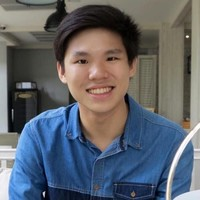
\includegraphics{./images/james_pic.jpg}

\textbf{Research Interest:}

James' research interest includes agricultural intelligence for
sustainable planning, including combining satellite imagery and machine
learning to help them monitor crop health, suggest how to optimize their
resources and warn them before the disaster is coming.

\bookmarksetup{startatroot}

\hypertarget{an-introduction-to-remote-sensing}{%
\chapter{An Introduction to Remote
Sensing}\label{an-introduction-to-remote-sensing}}

\begin{enumerate}
\def\labelenumi{\arabic{enumi}.}
\item
  Sensor

  \begin{enumerate}
  \def\labelenumii{\arabic{enumii}.}
  \tightlist
  \item
    Passive
  \end{enumerate}

\begin{verbatim}
1.  Use energy that is available

2.  Usually detecting reflected energy from the sun

3.  e.g. Human eye, camera, satellite sensor
\end{verbatim}

  \begin{enumerate}
  \def\labelenumii{\arabic{enumii}.}
  \setcounter{enumii}{1}
  \item
    Active

    \begin{enumerate}
    \def\labelenumiii{\arabic{enumiii}.}
    \item
      Have an energy source for illumination
    \item
      See through clouds
    \item
      e.g.~Radar, X-ray, LiDAR
    \end{enumerate}
  \end{enumerate}
\item
  Electromagnetic waves

  \begin{enumerate}
  \def\labelenumii{\arabic{enumii}.}
  \item
    Electromagnetic radiation (EMR) = Wave carry energy over time
  \item
    Energy carried by EMR waves = radiant energy
  \item
    Energy per unit of time = radiant flux
  \item
    Energy from the sun = incoming shortwave radiation or shortwave
    radiation
  \item
    Atmospheric Correction;

    \begin{enumerate}
    \def\labelenumiii{\arabic{enumiii}.}
    \item
      to remove atmosphere like cloud
    \item
      Big issue to deal with

      \begin{enumerate}
      \def\labelenumiv{\arabic{enumiv}.}
      \item
        Programming; detect cloud and estimate by other pictures
      \item
        Using active sensors like Synthetic Aperture Radar (SAR) to see
        through clouds, but the issue is about the accuracy of the
        outputs

        \begin{enumerate}
        \def\labelenumv{\arabic{enumv}.}
        \item
          emit the signal by polarization (single/dual)
        \item
          HH = emitted in horizontal (H) and received in horizontal (H)
        \end{enumerate}
      \end{enumerate}
    \end{enumerate}
  \item
    Color

    \begin{enumerate}
    \def\labelenumiii{\arabic{enumiii}.}
    \item
      Sky is blue; Sunlight is scattered by small wavelengths
    \item
      Moon sky is black; no atmosphere
    \item
      Ocean is blue; water absorb wavelength
    \end{enumerate}
  \end{enumerate}
\item
  Data

  \begin{enumerate}
  \def\labelenumii{\arabic{enumii}.}
  \item
    Format - Raster

    \begin{enumerate}
    \def\labelenumiii{\arabic{enumiii}.}
    \tightlist
    \item
      common file types: BIL, BSQ, BIP, GeoTIFF
    \end{enumerate}
  \item
    Resolutions

    \begin{enumerate}
    \def\labelenumiii{\arabic{enumiii}.}
    \item
      Spatial: range between 10 cm and several km

      \begin{enumerate}
      \def\labelenumiv{\arabic{enumiv}.}
      \tightlist
      \item
        (e.g.~20cm or 30m)
      \end{enumerate}
    \item
      Spectral: the number of bands it records data

      \begin{enumerate}
      \def\labelenumiv{\arabic{enumiv}.}
      \tightlist
      \item
        spectral signature - creating from values for each wavelength
        across the electromagnetic spectrum
      \end{enumerate}
    \item
      Temporal = the time it revisits

      \begin{enumerate}
      \def\labelenumiv{\arabic{enumiv}.}
      \tightlist
      \item
        e.g.~daily, every 7 days, on demand
      \end{enumerate}
    \item
      Radiometric = identify differences in light or reflectance

      \begin{enumerate}
      \def\labelenumiv{\arabic{enumiv}.}
      \tightlist
      \item
        e.g an 8 bit sensor has values between 0 and 255 (256 possible
        values), an 11 bit sensor has values between 0 and 2047
      \end{enumerate}
    \end{enumerate}
  \item
    Color

    \begin{enumerate}
    \def\labelenumiii{\arabic{enumiii}.}
    \item
      True color: human can see e.g.~red, blue, green
    \item
      False color: including many bands human can't see
    \end{enumerate}
  \item
    Satellite imagery

    \begin{enumerate}
    \def\labelenumiii{\arabic{enumiii}.}
    \item
      MODIS - 500 m
    \item
      Landsat - 30 cm
    \end{enumerate}
  \end{enumerate}
\end{enumerate}

\bookmarksetup{startatroot}

\hypertarget{landsat-sensor}{%
\chapter{Landsat Sensor}\label{landsat-sensor}}

\hypertarget{spectral-bands}{%
\subsection{Spectral bands}\label{spectral-bands}}

\begin{itemize}
\tightlist
\item
  VIS, NIR
\end{itemize}

\hypertarget{characteristics}{%
\subsection{Characteristics}\label{characteristics}}

\begin{itemize}
\tightlist
\item
  30m spatial resolution, revisit period is 16 days
\end{itemize}

\bookmarksetup{startatroot}

\hypertarget{references}{%
\chapter*{References}\label{references}}
\addcontentsline{toc}{chapter}{References}

\hypertarget{refs}{}
\begin{CSLReferences}{0}{0}
\end{CSLReferences}



\end{document}
